\chapter{Numerical Method}
\label{sec:methods}
In the previous chapter, the basics of plasma physics and the mathematical tools required to analyze plasma dynamics were introduced. Solving the equations of motion for the millions of plasma particles analytically is impractical, this section will outline the Particle-in-Cell (PiC) algorithm as a framework for computer simulation of plasma. A method for implementing photoelectron emission from conducting surfaces is emphasized. First, a general description of the PiC algorithm is introduced as well as the stability criteria of the algorithm. Then the implementation of the PiC algorithm in the PINC framework is discussed with emphasis on the implementation of object charging in plasma. Finally, a method for implementing photoelectron emission into the PINC object module is presented.

\section{Particle In Cell algorithm}
The particle in cell algorithm is a method used in computational plasma physics to analyze large systems of many particles in a computationally efficient manner. This is achieved by the introduction of super particles, computational particles, that represent many real particles, then interpolating the forces acting on these super particles to a spatial grid.\\
There are three main ways of simulating the forces acting on a system particles. The particle-particle method (PP) where forces are computed between individual particles. The particle-mesh method (PM) where the forces between the particles are computed as field quantities on the spatial mesh. And the particle-particle-mesh method (PPPM or $P^3M$), which is a combination of the two earlier methods \parencite{Birdsall2004}.\\
By far the simplest method computationally is the PP method. However, since all forces between each individual pair of particles are computed, the method is also the most computationally expensive. If the system of interest contains $N_p$ particles, then the number of operations scale as $\mathcal{O}(N^2_p)$ \parencite[p.20]{Hockney1988}. It is therefore impractical to use the PP method for all but the simplest systems, even on highly parallel High Performance Computers (HPC) available today.\\
The PM method computes the forces of a system as field quantities, first by assigning the charges in the system to the mesh by some method, then solving Poisson's equation on the mesh, then computing the forces on the mesh points and interpolating to the individual particles. This method is therefore faster, but usually not as accurate as computing the forces on all particle pairs directly. With $N_g$ grid points, the complexity of this method scales as $\mathcal{O}(N_g \log{N_g})$ \parencite{Hockney1988} thus making this method much more applicable to larger systems than the PP method.

\begin{figure}[h!]
    \centering
    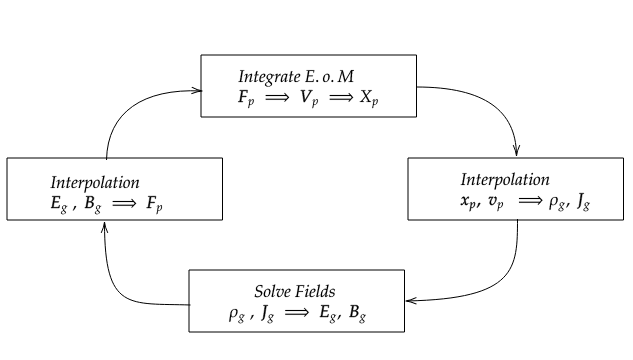
\includegraphics[scale=0.6]{figures/ReferenceFigures/PiC.png}
    \caption{Particle in cell compute cycle}
    \label{fig:pic}
\end{figure}

The PiC algorithm is an example of the PM method, figure \ref{fig:pic} shows an overview of a computational cycle for each timestep in the PiC algorithm. Beginning at the box on the right in the figure, a distribution of $N_p$ particles with position $\vb{x}_p$ is interpolated to get the charge $\rho_g$ and current density $\vb{j}_g$ at the surrounding grid points. The two most common methods for this interpolation is the Nearest Grid Point (NGP) scheme, and Cloud in Cell (CIC) scheme.\\
Once the charge and current densities are known on the grid, the next step is to solve for the $\vb{E}$ and $\vb{B}$ fields. This is accomplished by solving Maxwell's equations at the grid points

\begin{subequations}
    \begin{align}
        Gauss's\; Law: \nabla \cdot \vb{E} &= \frac{\rho}{\epsilon_0} \label{eq:gauss} \\
        Gauss's\; Law\; for\; magnetism: \nabla \cdot \vb{B} &= 0 \\
        Maxwell - Faraday's\; equation: \nabla \cross \vb{E} &= - \pdv{\vb{B}}{t}\\
        Ampere's\; Law: \nabla \cross \vb{B} &= \mu_0 \left(\vb{J} + \epsilon_0 \pdv{\vb{E}}{t} \right)
    \end{align}
\end{subequations}

Where $\rho$ is the charge density, $\epsilon_0$ is the vacuum permittivity, $\mu_0$ is the vacuum permeability, and $\vb{E}$ and $\vb{B}$ are the electric and magnetic fields respectively. With the electric and magnetic field computed at the grid nodes, the force on each super particle is computed from Lorentz's force equation and interpolating back to the position of the super particles. Using some numerical integrator the new position and velocity of the super particle is updated from the computed forces, and the cycle can then be repeated for the next timestep. 

\section{Particle in Cell implementation in PINC}
In this section, we discuss the methods implemented in PINC that are required for the main PiC compute cycle described in figure \ref{fig:pic} with focus on the particular schemes used in this thesis. The scheme used in PINC for integrating the equations of motion are presented, followed by the multigrid field solver, and finally the particle weighting scheme is discussed. PINC is the work of many researchers, but have been mainly implemented by Sigvald Marholm, Gullik Killie \parencite{Killie}, Vigdis Holta \parencite{Holta2018}, and Steffen Brask \parencite{Brask2018}. Significant contributions have also been made by Jan Deca, who implemented the module for object charging in PINC. This module will be discussed in more detail later in this chapter. 

\subsection{Integration of the equations of motion}
Planet Mercury possesses and internal magnetic field, as such the plasma surrounding the planet is magnetized. To solve for the motion of magnetized plasma, the Boris algorithm is used to integrate the equations of motion. The Boris algorithm is a variant of the well known leapfrog method, in which the position and velocity of a particle is updated at half timesteps in staggered fashion. Like the leapfrog method, the Boris algorithm is an energy conserving integrator; the merits of the Boris algorithm as the de facto particle mover is further expanded upon in the publication \parencite{Qin2013}.
\\
Using the same notation as defined in \parencite{Birdsall2004} the Lorentz force is discretized as 

\begin{subequations}
    \begin{align}
        \frac{\vb{x}^{t+\Delta t}_p - \vb{x}^t_p}{\Delta t} &= \vb{v}^{t + \frac{\Delta t}{2}} \\
        \frac{\vb{v}^{t+\Delta t}_p - \vb{v}^{t-\Delta t}_p}{\Delta t} &= \frac{q_s}{m_s} \left(\vb{E}_p + \frac{\vb{v}^{t+\Delta t}_p - \vb{v}^{t-\Delta t}_p}{2} \cross \vb{B}_p \right) \label{eq:borizVel}
    \end{align}
\end{subequations}

In the Boris algorithm equation \eqref{eq:borizVel} is decomposed into a series of updating steps. First, half the acceleration is added, then the intermediary velocity vector is rotated due to the external magnetic field $\vb{B}$, and finally the second half of the acceleration is added.

\begin{subequations}\label{eq:borisNewVel}
    \begin{align}
        \vb{v}^{-} &= \vb{v}^{t-\Delta t}_p + \frac{q_s}{m_s} \vb{E}_p \frac{\Delta t}{2} \\
        \vb{v}^{'}_p &= \vb{v}^{-}_p + \vb{v}^{-}_p \cross \vb{T} \\
        \vb{v}^{+}_p &= \vb{v}^{-}_p + \vb{v}^{'}_p \cross \vb{S} \\
        \vb{x}^{t+\Delta t}_p &= \vb{v}^{+}_p + \frac{q_s}{m_s} \vb{E}_p \frac{\Delta t}{2} 
    \end{align}
\end{subequations}

Where the rotational parameters $\vb{T}$ and $\vb{S}$ are expressed as

\begin{subequations}\label{eq:BrotParams}
    \begin{align}
        \vb{T} &= \hat{\vb{B}}_p \cdot \tan\left(\frac{q_s \Delta t}{2m} B_p \right) \\
        \vb{S} &= \frac{2 \vb{T}}{1 + \norm{\vb{T}}^2}. 
    \end{align}
\end{subequations}

Where $\hat{\vb{B}}_p$ is the magnetic unit vector acting on particle $p$. Equations \eqref{eq:borisNewVel} are equally suited for plasmas with time varying magnetic fields as for electrostatic plasma with a constant external magnetic field. Since PINC is an electrostatic model, equations \eqref{eq:BrotParams} is solved once before the main time loop, then applied to each call to the mover method.

\subsection{Field Solver}
Several field solvers exists in PINC, in this thesis the multigrid solver developed by Killie \parencite{Killie} has been used. The multigrid solver is an iterative method; the basic principle of the method in a PiC context is to solve Poisson's equation first on a coarse grid, then using the solution on the course grid as a guess, solve the equation again for a finer grid. The solution for the coarse grid speeds up the solution for the finer grid, reducing the total computational time required to converge to an accurate solution. 
\\
There are three main types of multigrid solver, divided into the so called V-cycle, W-cycle and F-cycle, defined by when the algorithm should use a coarser or finer mesh than used in the previous iteration. Multigrid solvers are highly flexible, and many researchers have spent considerable effort in order to optimize the number of iterations \insertref{Multigrid, Trottenberg et al}, highly optimized multigrid solvers have a local complexity given by $\mathcal{O}(N_g)$, with a global complexity of $\mathcal{O}(N_g log(N_g))$ when using domain decomposition like in the case of PINC \insertref{Trottenberg2020}.
\\
As described earlier, the multigrid method solves Poisson's equation in PINC. Strictly speaking, the solution to Gauss's law, equation \eqref{eq:gauss} is solved. In PINC however, electrostatic plasma is assumed, in this case the electric field is irrotational, i.e. $\nabla \cross \vb{E} = 0$ and the electric field can then be represented as the gradient of a scalar potential field $\vb{E} = \nabla \phi$.  Substituting the potential field back into Gauss's law, equation \eqref{eq:gauss} we have Poisson's equation

\begin{equation}\label{eq:poisson}
    \nabla^2 \phi = \frac{\rho}{\epsilon}
\end{equation}

In PINC this equation is solved iteratively using the Gauss-seidel method. Gauss-Seidel discretizes \eqref{eq:poisson} using the Forward-Time Central-Space (FTCS) finite difference scheme. In one spatial dimension, the electric field in terms of the potential becomes

\begin{equation}\label{eq:Ediscrete}
    \vb{E}_g = \frac{\phi^{n+1}_g - \phi^{n-1}_g}{2\Delta x}
\end{equation}

and Poisson's equation, equation \eqref{eq:poisson}, becomes

\begin{equation}\label{eq:poissonDescrete}
    \frac{\phi^{n+1}_g - 2\phi^n_g + \phi^{n-1}_g}{{\Delta x}^2} = - \frac{\rho_g}{\epsilon}
\end{equation}


Where the subscript g implies the evaluation of $\phi$ at grid points, and the superscript p denotes the grid node index. Analogous expressions can be formed in two and three spatial dimensions.

\subsection{Particle weighting}
In the particle in cell method particles can exist anywhere in the continuous spatial computational domain, but forces and charge densities are calculated at discrete grid points \parencite[chapter 2.6]{Birdsall2004}. Historically, the NGP method and CIC method are used to weight computational particles to the grid. Higher order schemes exists, such as Quadratic Splines (QS) and Cubic Splines (CS), see \parencite{Okuda1979} for an overview on the usage of higher order weighting schemes in plasma simulation. In PINC the CIC method is used to weight particle parameters to the grid. Using similar notation as Verboncoeur \parencite{Verboncoeur2005} the weighting function is defined as 

\begin{equation}\label{eq:weightFunc}
    \vb{w}_{i,j,k} = \vb{x}_p - \vb{X}_{i,j,k}
\end{equation}

Where $\vb{x}_p$ is the position of particle p, and $\vb{X}_{i,j,k}$ is the position of the nearest grid point closest to the origin. Using equation \eqref{eq:weightFunc}, the charge distribution of particle p to a two dimensional grid can be found as

\begin{subequations}
    \begin{align*}
        Q_{i,j} &= q_p \, (1 - w_i) \, (1 - w_j) \\
        Q_{i+1,j} &= q_p \, w_i \, (1 - w_j) \\
        Q_{i,j+1} &= q_p \, (1 - w_i) \, w_j \\
        Q_{i+1,j+1} &= q_p \, w_i \, w_j 
    \end{align*}
\end{subequations}

With similar equations for the three dimensional case can be found from equation \eqref{eq:weightFunc}. From the charge distribution found above, the charge density can be found directly by dividing the charge distribution by the volume of a computational cell, i.e 

\begin{equation*}
    \rho_{i,j,k} = \frac{Q_{i,j,k}}{V_{i,j,k}}
\end{equation*}

From the charge density and current density, PINC computes the electric and magnetic field using the multigrid field solver module.

\section{Simulation stability and constraints}

\subsection{Spatial resolution}
In PINC, and in other particle in cell codes, particles move in continuous space, but their macroscopic properties are projected to a discrete grid. Representing continuous variables on a discrete grid leads to numerical instability called finite grid instability \parencite[section 5.1.]{Lapenta2011}. The analysis of finite grid instability is beyond the scope of this thesis, a rigorous mathematical description of finite grid instability can be found in for example \textit{Plasma physics via computer simulation} \parencite{Birdsall2004}. The most important result of these analyses is that the grid spacing $\Delta x$ must satisfy the condition

\begin{equation}\label{eq:GridSize}
    \frac{\Delta x}{\lambda_D} < C
\end{equation}


Where C is some constant dependent on the discretization scheme used. In the case of the CIC scheme, the constant C is approximately equal to $\pi$. Failure to meet this condition in a PIC simulation leads to unphysical heating of the plasma. Equation \eqref{eq:GridSize} must therefore be satisfied in all directions of the full computational domain to ensure conservation of energy.

\subsection{temporal resolution}
In PINC, the boris algorithm is used for particle pushing. The boris algorithm is an explicit forward time integration scheme, and as such simulations run with PINC must satisfy temporal stability constraints associated with such schemes. A Von Neumann stability analysis of a harmonic oscillator without an external magnetic field given by the following equation \parencite{Hockney1988}, \parencite{Birdsall2004}, \parencite{Lapenta2011} 

\begin{equation}\label{eq:harmonicOscillator}
    \frac{q_s}{m_s} \vb{E}_p(\vb{x}_p) = - \Omega^2 \vb{x}_p
\end{equation}

leads to the equation 

\begin{equation}
    \left(\frac{\Omega \Delta t}{2} \right)^2 = \sin^2{\left(\frac{\omega_N \Delta t}{2}\right)}
\end{equation}

Where $\omega_N$ is the numerical oscillation frequency. For values outside the range [-1,1] the sine function has only complex solutions, thus for timesteps $\Delta t$ where  $\Omega \Delta t > 2$ is true, the numerical oscillation frequency will be complex. Any practical simulation of the harmonic oscillator will therefore become unstable due to unbounded numerical heating. Thus, the finite time stability criteria can be expressed as

\begin{equation}
    \Omega \Delta t < 2
\end{equation}

In this thesis, for solar wind simulations, the frequency $\Omega$ that needs to be resolved is typically the electron oscillation frequency of the cold solar wind plasma. 


\subsection{The CFL condition}
The Courant–Friedrichs–Lewy condition, or CFL condition, is a stability criteria linking the finite timestep and grid step, $\Delta t$ and $\Delta x$ respectively. The condition must be met everywhere in the computational domain if the explicit integrator in PINC is to converge to a solution.

In \insertref{See Steffens master thesis..} a common formulation of the condition is given as

\begin{equation}
    \frac{\Delta x}{\Delta t} > C
\end{equation}

Where C is some characteristic speed. The constant C is solver scheme dependent, and is often set as $C = 1$ for explicit schemes; in PINC this qualitatively means that a particle is restricted to move by maximum one computational cell per timestep as the length scale is normalized to the grid step size.

\section{The PINC Object module}
The object module in PINC contains a set of functions and data structures necessary for simulating objects immersed in plasma. It was developed primarily by Jan Deca and Sigvald Marholm as a part of a collaboration between the University of Oslo and University of Colorado Boulder. In the object module, spacecraft-plasma interations are simulated using the same Capacitance Matrix method outlined by Miyake and Usui in developing the PIC code EMSES (the ElectroMagnetic Spacecraft Environment Simulator) \parencite{Miyake2009}. 

In this section the method used in PINC for defining objects on a structured Cartesian grid is discussed in brief; a description of the \textit{Grid} data structure and associated functions in PINC is also introduced as all scalar and vector fields are represented in PINC using this data structure, including conducting objects which are defined as scalar fields. The capacitance matrix method is then outlined, with an emphasis on the equations that have been implemented in PINC. 


\subsection{Representing objects on a grid}
In the PINC object module, conducting objects are represented as points on the Cartesian computational grid, and stored in an input HDF5 (Hierarchical Data Format) file. Internally in PINC, this file is converted to a PINC \textit{Grid} structure instance and is stored as a subset of the \textit{Object} data structure which additionally contains data on which nodes are internal to the object, which nodes are on the surface, and data required in photoemission computations. Required data for photoemission in the \textit{Object} structure will be described in the later section on implementation of photoemission in PINC.

The PINC \textit{Grid} structure is a generalized data structure that stores N-dimensional data in a flat manner. The values on the grid is stored in a lexicographical manner; the elements of the three dimensional array is then represented in PINC as

\begin{equation*}
    (0,0,0), \, (1,0,0), \,, \, (2,0,0), \, ... \, , \, (0,1,0) \,, \, (1,1,0) \,, \, (2,1,0) \,, \, ...
\end{equation*}

Objects in PINC are thus stored as 1 by N arrays representing scalar fields, where N is the total number of grid points in the computational domain. The \textit{Grid} structure additionally contains a data field called \textit{sizeProd}, that allows for converting between Cartesian grid point coordinates and the index of value in the array: This field is an array that contains the cumulative product of the number of grid points along each axis in the computational domain. Thus, the index $p$ of the value of a \textit{Grid} structure located at the Cartesian coordinates $(x,y,z)$ is represented as

\begin{equation}\label{eq:PINCindex}
    p = x \cdot \text{sizeProd}[0] + y \cdot \text{sizeProd}[1] + z \cdot \text{sizeProd}[2]
\end{equation}

Traversing along an axis from a point with index $p$ of the \textit{Grid} structure, is then the simple matter of adding the corresponding element of the \textit{sizeProd} array to the index $p$. We will make use of this fact, along with equation \eqref{eq:PINCindex}, later in this chapter in creating an algorithm for photoemission on the surface of conducting objects. 


\subsection{The capacitance matrix method}
The general idea of the capacitance matrix method is to precalculate a capacitance matrix for each object immersed in the plasma in question. Applying the computed capacitance matrix, the charges due to super-particles impinging the object can be redistributed to the surface of the object, after redistribution of charges a charge density and electric potential correction is computed and spacecraft potential can be updated. super-particles located within the object are then removed from the computational domain after their charges have been redistributed. 

\todo{Create a new cycle diagram}
Figure \insertref{Updated PIC cycle diagram} shows a modified computational cycle for PINC when taking into account charge accumulation on the surface of a conducting object immersed in the plasma.

The capacitance matrix relates the potential $\phi$ and charge distribution $\rho$ as follows \parencite{Miyake2009}

\begin{equation}
    \rho_i = \sum^{N_G}_{j=1} A_{ij} \phi_j
\end{equation}

Where the matrix A represents the capacitance matrix, where i and j are the indices of the grid, and $N_G$ is the total number of grid points. Inverting matrix A, and defining $B \equiv A^{-1}$, the potential $\phi$ can be calculated as 

\begin{equation}
    \phi_i = \sum^{N_G}_{j=1} B_{ij} \rho_j
\end{equation}


After redistribution of charges, the charge density on the conducting body surface $\rho_s$ changes. The correction in potential on the spacecraft surface $\delta \phi_s$ can then be found from the charge density correction $\delta \rho_s$ as

\begin{equation}
    \delta \phi_{s,i} = \sum^{N_B}_{j=1} B_{ij} \delta \rho_{s,j}
\end{equation}

Where $N_B$ is the total number of surface nodes, and $N_B < N_G$. By forming a subset of matrix B with the values associated with the surface nodes, with $N_B$ rows and columns, and inverting this matrix the charge density correction on the surface can be found

\begin{equation}\label{eq:SCchargeCorr}
    \delta \rho_{s,i} = \sum^{N_B}_{j=1} C_{ij} \delta \phi_{s,j}
\end{equation}

Where the matrix $C$ is the inverted sub matrix of B. Qualitatively $C$ is the capacitance matrix of the conducting surface. In the PINC object module, matrix $C$ is constructed and stored before the main simulation loop begins by placing a unit charge on each grid point defining the conducting object surface, setting all other grid points to zero charge, and then solving for the potential: This forms the sub matrix of matrix $B$ which can then be inverted to find the surface capacitance matrix $C$, details of this implementation are found in appendix \ref{sec:ObjectCode}.

In the simulation time-loop of PINC, after the potential has been updated, but before charges have been distributed to the surface, the surface potential of the conducting body $\phi_{s,j}$ is not the same value for all values of j and is therefore not at an equipotential. 

The correction in potential in terms of the equipotential $\phi_c$ of the surface is given by

\begin{equation}\label{eq:SCphiCorrEqui}
    \delta \phi_{s,j} = \phi_c - \phi_{s,j}
\end{equation}

Substituting equation \eqref{eq:SCphiCorrEqui} into equation \eqref{eq:SCchargeCorr}, the charge density correction equation becomes

\begin{equation}\label{eq:SCrhoCorrNew}
    \delta \rho_{s,i} = \sum^{N_B}_{j=1} C_{ij} (\phi_c - \phi_{s,j})
\end{equation}

The equipotential $\phi_c$ is unknown in equation \eqref{eq:SCrhoCorrNew}; by using the fact that charges must be conserved when impinged charges are redistributed to the object surface, the equipotential can be calculated. Conservation of charge takes the form

\begin{equation}\label{eq:ConsSurfCharge}
    \sum^{N_B}_{i=1} \delta \rho_{s,i} = 0
\end{equation}

Substituting equation \eqref{eq:SCrhoCorrNew} into equation \eqref{eq:ConsSurfCharge}, $\phi_c$ can be computed as

\begin{equation}\label{eq:Equipotential}
    \phi_c = \frac{\sum_i \sum_j C_{ij} \phi_{s,j}}{\sum_i \sum_j C_{ij}}
\end{equation}

In the conducting object run mode of PINC, after a first pass of the multigrid Poisson solver, equations \eqref{eq:SCrhoCorrNew} and equation \eqref{eq:Equipotential} are solved to redistribute absorbed charged particles, a new pass with the Poisson solver then solves the new potential field using the correction to the charge density field. Details on the implementation of these equations in PINC can be referenced by contacting the 4DSpace group at the University of Oslo for access to the PINC code repository.

\newpage

\section{Implementing photoemission in PINC}

Photoelectric emission by sunlit spacecraft surfaces contribute significantly to the overall charge of a spacecraft. In fact, in normal conditions in geosynchronous orbits, the photoelectron flux exceeds that of the ambient electrons \parencite{Lai2006}. When there is a net outgoing current flux, spacecraft charge to to a positive voltage. In order to simulate spacecraft charging using PINC, it is then necessary to implement photoelectric emission. In this section the photoemission method implemented as part of this thesis is presented. 


\begin{figure}[h!]
    \centering
    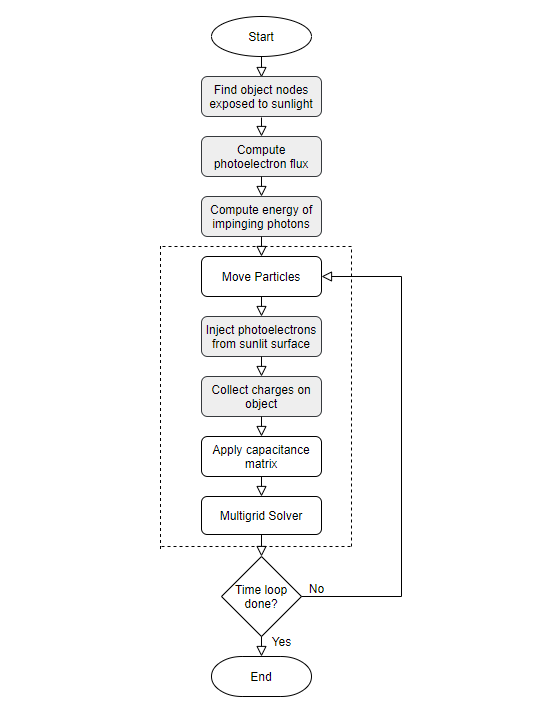
\includegraphics[width=12
    cm, height=15cm]{figures/photoemission.PNG}
    \caption{Flowchart describing the photoemission algorithm}
    \label{fig:photoemission}
\end{figure}

The flowchart shown in figure \ref{fig:photoemission} describes the general flow of PIC method as implemented in PINC when the photoemission modules developed for this thesis are included. Processes shown in the diagram are on a function level in the code, with processes colored grey describing functionality that needed to be implemented in PINC. The details of the implementation of these processes are shown later in this section. The functions placed within the stippled box are carried out for each iteration of the PIC time loop; since these functions are called with a greater frequency, it is vital that they are computationally efficient.

In addition to the functions described in the figure \ref{fig:photoemission}, the initialization function of the object structure in PINC was expanded to read input parameters required for the new photoemission functions. To facilitate ease of use, and to make the code more easily readable, function pointers were added such that the functions for computing photoelectron flux and photoelectron injection could be specified as part of an input file. 


\subsection{Identifying sunlit surfaces}

To be able to simulate photoemission, our code needs to know which surfaces the photoelectrons are supposed to be emitted from. As discussed in the previous section on the PINC object module, PINC has no "knowledge" on what faces make up the surface of an object embedded in the computational domain. Thus, it is necessary to locate the object nodes that are exposed to direct sunlight.

Two different functions were developed to find these surface nodes, which function to run is dependent on which algorithm selected for injecting photoelectrons into the computational domain.

The method for finding the surface nodes directly exposed to sunlight has been programmed with the assumption that photons travel in the same direction as the x axis of the domain to reduce the complexity of the code. 

Beginning at the node with index 0 of the domain, the code steps along the x direction checking whether each node index is an element of the array containing all object surface nodes. When the node index matches the index of a surface node, that index is stored in the object structure, and the loop stepping along the x axis is exited. The loop of stepping down the x axis is then repeated for each node along the y and z axis until the function has iterated through each "column" normal to the YZ plane. If a surface node is not located in a column parallel to the x axis, the function simply continues to the next column.

This function can be visualized as analogous to mapping the topology of the bottom of a lake by sinking a weight attached to a rope from the surface of the lake, and measuring the wetted length of the rope when the weight reaches the bottom.


\begin{minipage}{\linewidth}
\begin{lstlisting}[language=C, caption={Pseudo code for finding sunlit object surface nodes},
label={lst:sunlitNodes}]
void oFindAllSunlitNodes(...){

    ... define and initialize variables ...

    for(int k = 0; k<size[z]; k++){
    
        for(int j = 0; j<size[y]; j++){
                
            int flag = 0;
            for(int i = 0; i<size[x]; i++){
                
                index = i*sizeProd[1] + j*sizeProd[2] + k*sizeProd[3];
                for(int n = 0; n < nSurfaceNodes; n++){
                    
                    surfNode = surface[n];
                    if(surfNode == index){
                        ... append index to exposed node array ...
                        flag = 1;
                        break;
                    }
                    
                if(flag) break;
                
                }
            }
        }
    }
}
\end{lstlisting}
\end{minipage}

\vspace{1cm}
Listing \ref{lst:sunlitNodes} shows the basic structure of the function described above. Each column normal to the YZ plane is stepped down using the "size" array that stores the number of nodes along each axis of the domain. The linear index of the node is then found using equation \eqref{eq:PINCindex} and compared with the indices of surface nodes stored in the "surface" array. 

The surface node array is initialized by a function that computes the object capacitance matrix, which is called before the sunlit surface nodes are found. In the photoelectron injection function, the indices of the sunlit nodes can then be converted into Cartesian coordinates with a helper function using the "sizeProd" array. 

A similar function to listing \ref{lst:sunlitNodes} finds the subset of object surface nodes that are used for photoelectron injection by filling cells adjacent to the emitting surfaces.
Since PINC does not store data defining cells, and each node is surrounded by 8 computational cells, it is necessary to consistently pick which cell to fill with photoelectrons. For a surface node with linear index $p$ located at grid points $[i,j,k]$ we choose the cell to be filled by the nodes $[i-1,j,k], [i-1,j+1,k], [i-1,j,k+1], [i-1,j+1,k+1], [i,j,k], [i,j+1,k], [i,j,k+1], [i,j+1,k+1]$. In PINC we have defined the sunlit surface of the object by the projection of the object onto the YZ plane, therefore for a cell to be "on" the surface of the object we also require that the vertices $[i,j,k], [i,j+1,k], [i,j,k+1], [i,j+1,k+1]$ of the cell are also surface nodes.

\begin{figure}[h!]
    \centering
    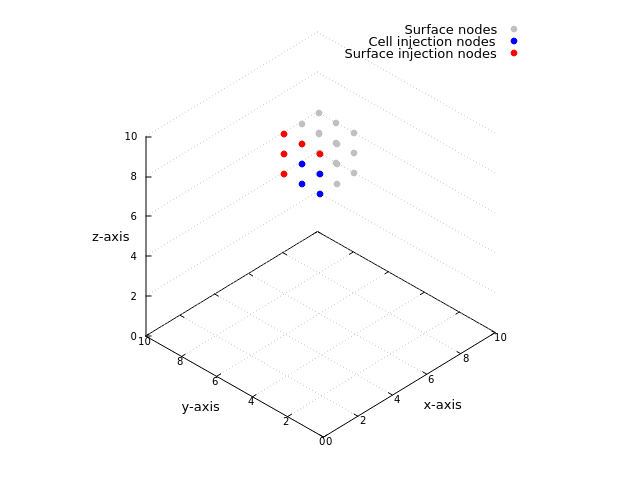
\includegraphics[scale=0.6]{figures/ReferenceFigures/nodes.png}
    \caption{Surface nodes on a box exposed to sunlight}
    \label{fig:sunlitNodes}
\end{figure}

Figure \ref{fig:sunlitNodes} is a visual representation of why this condition must be met for nodes used for the cell filling injection algorithm. It shows the surface nodes of a 2 unit by 2 unit box inside a computational box of 10 x 10 x 10 nodes where the sunward direction is along the negative X axis. Nodes marked in blue are nodes used for photoelectron injection by cell filling, the surface injection algorithm uses the nodes colored \textbf{both} red and blue. Cells defined by nodes colored red are not adjacent to the sunlit surface in the XY plane.

Another condition is necessary to avoid selecting cells that are part of the interior of the object; we further stipulate that for nodes $[i-1,j,k], [i-1,j+1,k], [i-1,j,k+1], [i-1,j+1,k+1]$ a maximum of three are either surface nodes \textbf{or} interior nodes of the object.


\begin{minipage}{\linewidth}
    \begin{lstlisting}[language=C, caption={C pseudocode for finding cells adjacent
    to sunlit object surfaces},
    label={lst:sunlitCells}]
    
    void oCellFillingNodes(...){
        
        ... variable definitions and initialization ...
    
        for(long int i = surfaceOffset[a]; i<surfaceOffset[a+1]; i++){
                    
            int nObjNode = 0;
            int yzPlane = 0;        
          
            //cell nodes
            long int p = surface[i];
            long int pu = p + sizeProd[3];
            long int plu = p + sizeProd[2] + sizeProd[3];
            long int pl = p + sizeProd[2]; 
            long int po = p - sizeProd[1];
            long int pou = p - sizeProd[1] + sizeProd[3];
            long int poul = p - sizeProd[1] + sizeProd[3] + sizeProd[2];
            long int pol = p - sizeProd[1] + sizeProd[2];
        
            for(int j = interiorOffset[a]; j < interiorOffset[a+1]; j++){
                long int intNode = interior[j];
                if(po == intNode || pou == intNode ||
                   poul == intNode || pol == intNode){
                    nObjNode++;
                }
            }
        
            for(int j = surfaceOffset[a]; j < surfaceOffset[a+1]; j++){
                long int surfNode = surface[j];
                if(po == surfNode || pou == surfNode || 
                   poul == surfNode || pol == surfNode){
                    nObjNode++;
                }
        
                if(p == surfNode || pu == surfNode || 
                   plu == surfNode || pl == surfNode){
                    yzPlane++;
                }
            }
        
            if(yzPlane == 4 && nObjNode < 8){
                ... store index p as an emitting node for cell filling ...
            }
        }
    }
    \end{lstlisting}
\end{minipage}


A C style pseudocode implementation of these conditions are given in listing \ref{lst:sunlitCells}; the "surfaceOffset" stores the number of surface nodes for object "a", then the defined cell vertices are stored. The linear index of these vertices are then compared against the "surface" array and "interior" array. We then check whether the cell has a face on the surface of the object, and that the cell is \textbf{not} an interior cell.


\subsection{Photoemission current and photoelectron energy}\label{subsection:CurrentDensity}
Two methods have been developed in PINC for finding the temperature, and flux of photoelectrons from sunlit object surfaces. The first method has been previously discussed in chapter \cref{sec:theory}; integrating Planck's law over a frequency band, allows both the photoelectron flux and temperature to be calculated. 

For some objects, especially spacecraft, the photoelectric current, and the temperature of the emitted electrons are known a priori to our simulation. These values can then be specified as a input parameters to PINC.

The number of super particles to inject per timestep into each cell adjacent to the sunlit surface is directly computed from the photoelectron current flux \parencite{Deca2013}

\begin{equation}\label{eq:NPHelectrons}
    N_{inject} = j_{ph} \frac{dA \cdot dt}{q_{part}}
\end{equation}

Where $N_{inject}$ is the number of super particles to inject into each photoemitting cell, $dA$ is the area of a computational cell, $dt$ is the simulation timestep, and $q_{part}$ is the charge of one computational particle. The charge on one particle is calculated as

\begin{equation}
    q_{part} = \frac{\rho \, e \, V_{cell}}{N_{p,cell}}
\end{equation}

where $\rho$ is the electron density, $V_{cell}$ is the volume of the cell, and $N_{p,cell}$ is an input parameter specifying the number of particles per computational cell. Equation \eqref{eq:NPHelectrons} can be rewritten to calculate the total number of photoelectrons ejected per timestep. Since several photoelectron injection methods have been analyzed for this thesis, the total photoelectron flux per timestep is the form that has been implemented into PINC

\begin{equation}
    N_{total} =  \frac{j_{ph} \cdot A \cdot dt}{q_{part}}
\end{equation}

where the total area of the sunlit object surface $A$ has been used instead of the cell surface area. These particles are then injected into the computational domain with velocity sampled from a Maxwellian plasma with an average temperature given by the input parameters. Which method PINC uses for finding photoelectron flux is specified as a flag in the simulation input file.  

\subsection{Integrating Planck's law}

The photoelectron flux of a sunlit object is dependent on the material composition of the sunlit surface. Surfaces with a lower work function tend to eject more photoelectrons.

Similarly, the photoelectron flux of a sunlit surface is proportional to the distance from the surface to the sun. Since the power output of the sun follows an inverse square law with the square of the distance from the sun. The closer the spacecraft is to the sun in its orbit the higher the number of photons with energy greater than the work function strike the surface of the spacecraft. Both these factors need to be accounted for in order to make simulating spacecraft charging in sunlight as general as possible. 

The number of photoelectrons emitted is however not equal to the number of impinging photons with energy higher than the surface work function. Both the reflectance of the surface, and the photoelectron yield of the surface material significantly reduce the photoelectron flux. Reflectance and photoelectron yield are both dependent on the energy of incoming photons, but are assumed to be constant in this thesis.

Thus, to compute the photoelectron flux for a particular spacecraft, Planck's law must be integrated in the frequency band from the work function frequency, to infinity before the main particle-in-cell loop is started. The photoelectron flux can then be directly computed from the power received by the spacecraft, as long as the surface area exposed to the sun and work function of the spacecraft material surface is known. These variables, in addition to the material photoelectron yield and reflectance, can be given as inputs to our simulation.

Integrating Planck's additionally allows the average kinetic energy of the emitted photoelectron to be calculated, dividing the total radiation energy absorbed per timestep by the total photoelectron flux.

Several methods for numerically integrating Planck's law efficiently exists. In this thesis, the method settled on is based on the paper by Widger and Woodall \parencite{Widger1976}. A overview of the method presented in that paper, and the implementation in PINC as C pseudocode will now be given.

First, to simplify the integrals, Planck's law is recast in terms of the wavenumber ($cm^{-1}$) $\nu$ rather than the frequency of radiation. Planck's law then takes the form

\begin{equation}\label{eq:PlanckNu}
    B(T) = C_1 \int^{\infty}_{\nu} \nu^3 \left(\exp{\frac{C_2 \nu}{T}} - 1 \right) d \nu
\end{equation}

Where B(T) is the radiance, given in units of $W cm^{-2} Sr^{-1}$, T is the absolute temperature in Kelvins, and $C_1$ and $C_2$ are the first and second radiation constants respectively.

Letting $x = C_2 T^{-1} \nu$, equation \eqref{eq:PlanckNu} can be rewritten as 

\begin{equation}\label{eq:PlanckX}
    B(T) = C_1 C_2^{-4} T^4 \int^{\infty}_x \frac{x^3}{\exp{x} - 1} dx
\end{equation}

The integrand in equation \eqref{eq:PlanckX} can be expanded in a series form, substituting that series into equation \eqref{eq:PlanckX} and integrating by parts, equation \eqref{eq:planckX} becomes

\begin{equation}\label{eq:PlanckSum}
    \int^{\infty}_x \frac{x^3}{\exp{x} - 1} dx = \sum^{\infty}_{n=1} \exp{-n x} \left(x^2 n^{-1} + 3 x^2 n^{-2} + 6 x n^{-3} + 6 n^{-4} \right)
\end{equation}

$C_1$, $C_2$ and T are known constants in equation \eqref{eq:PlanckX}, and the infinite sum in equation \eqref{eq:PlanckSum} is straight forward to compute to some finite tolerance using a C function. The integral in \eqref{eq:PlanckSum} is computed in units of radiance $W m^2 Sr^{-1}$, the solid angle $\Omega$ of the photoemitting object with respect to the sun can be calculated as

\begin{equation*}
    \Omega = \frac{A_s}{r^2}
\end{equation*}

Where $A_s$ is the area of the sunlit surface, and $r$ is the radial distance from the center of the sun to the object. Multiplying the result of \eqref{eq:PlanckSum} by the solid angle of the object with respect to the sun, and the surface area of the sun, the power output in the frequency band above the work function of interest can be found. A similar integral to the one found in equation \eqref{eq:PlanckSum} can be constructed in terms of photons per second instead of Watts.

Computing the photons impinging on the surface per timestep does not however correspond to the amount of photoelectrons emitted by the sunlit surface. To compute the total photoelectron flux, the photon impinging rate must be multiplied by the surface material reflectance, and the photoelectron yield (number of electrons emitted per incoming photon above the work function of the material) as described in chapter \ref{sec:theory}.

\begin{minipage}{\linewidth}
\begin{lstlisting}[language=C, caption={Numerical integration of Planck's law in terms of photon flux}, label={lst:planck}]
void oPlanckPhotonIntegral(...){

  ... Variable and constant definitions and initialization ...
    
  for(int a=0; a<nObj; a++){
	//sigma[a] = ((double)sigma[a]) / (Planck * speedOfLight * 100.);
	double c1 = Planck * speedOfLight / Boltzmann;
	double x = c1 * 100. * (double)sigma[a]/temperature;
	double x2 = x * x;

	// decide how many terms of sum are needed
	double iterations = 2.0 + 20.0/x;
	iterations = (iterations < 512.) ? iterations : 512;
	int iter = (int)(iterations);
	// add up terms of sum
	double sum = 0.;
	for (int n=1; n<iter; n++) {
	  double dn = 1.0 / n;
	  sum += exp(-n*x) * (x2 + 2.0*(x + dn)*dn) * dn;
	}
	//result, in units of photons/s/m2/sr, convert to photons/timestep
	double kTohc = (Boltzmann * (double)temperature) / (Planck * speedOfLight);
	double solidAngle = (double)area[a] / pow(distFromSun,2.);
	radiance[a] = 2.0 * pow(kTohc,3.) * speedOfLight;
	radiance[a] = radiance[a] * sum;
	radiance[a] *= solidAngle * sunSurfaceArea;
	radiance[a] *= (1.0 - reflectance) * phYield;
	radiance[a] *= time;
  }
    
  ... Store radiance to object structure here ...

}
\end{lstlisting}
\end{minipage}

Listing \ref{lst:planck} shows a numeric implementation of equation \eqref{eq:PlanckX} and equation \eqref{eq:PlanckSum}. The original algorithm \parencite{Blackbody} has been converted from C++ code to C for compatibility with the PINC framework.


\subsection{Injection of photoelectrons}\label{subsec:injection}
The method selected for injecting a Maxwellian velocity distribution of electrons affect the accuracy of the results from a particle in cell simulation. Once the average kinetic energy of the photoelectrons has been calculated as seen in previous sections, a Maxwellian velocity distribution can be constructed from the average velocity. 

The position of the particles must also be distributed into the computational domain in such a way that the particles remain Maxwellian in their velocity distribution. Describing an accurate particle distribution function $f(\vb{x}, \vb{v}, t)$ is especially important for simulations with timescales longer than that that of the ion transit time, and for simulations that include Monte Carlo collision modules \parencite{Cartwright2000}.  

In the code developed for this thesis, three methods for injecting photoelectrons were analyzed; two methods based on injecting electrons directly from the surface nodes exposed to sunlight, and one method in which electrons were uniformly distributed in the computational cells adjacent to the emitting surfaces.

Later in this chapter, these injection algorithms are tested against the charging simulations of the Solar Probe plus presented in \parencite{Deca2013}.

\subsubsection*{Surface node injection}

The simplest method for injecting the photoelectrons from a surface, is by defining all object surface nodes exposed to sunlight as particle sources. The position of each emitted particle is computed as an "push" based on the Maxwellian velocity distribution from the position of each node:

\begin{equation}\label{eq:injection}
    x_i = x_{\text{node},i} + R \, v_i
\end{equation}

Where $x_{i,j}$ denotes the position component in the i direction of the injected particle, $x_{node,i}$ denotes the position of some node in the i direction, R is some random number on the interval $[0,1]$, and $v_i$ is the sampled velocity component in the i direction of the injected particle.

Two methods for sampling the Maximilian velocity distribution were analyzed; the first was based on the Box-Mueller algorithm \parencite{Deca2013}.

In the Box-Mueller algorithm, the tangential velocities are sampled from the bivariate Maxwell distribution:

\begin{equation}\label{eq:bivariateMaxell}
    f(v_{t1}, v_{t2}) = \left(\frac{m}{2 \pi k T}  \right) \exp \left(- \frac{m (v^2_{t1} + v^2_{t1})}{2 k T} \right)
\end{equation}

Whereas the normal component of the velocity is sampled from a half-Maxwellian distribution, described by the distribution function

\begin{equation}\label{eq:halfMaxwell}
    f(v_n) = \left(\frac{m}{2 \pi k T}\right)^{1/2} \exp \left(- \frac{m v^2_n}{2 k T} \right)
\end{equation}

The bivariate distribution is implemented in PINC by sampling a bivariate Gaussian distribution with a variation equal to the average thermal velocity of the photoelectrons. The normal component of the photoelectron velocity is sampled from a univariate Gaussian distribution, also with a variation equal to the average thermal velocity, and rejecting the negative velocities (pointing into the object).

The second node injection method implemented similarly distributed emitted particles as a partial push using equation \eqref{eq:injection}. The method differs in how the velocity distribution of the particles were sampled. First, the speed of the electron is sampled from a univariate Gaussian distribution and the velocity of the particle is initialized as parallel and opposite to the direction of the sun. Then, a rotation matrix is formed from subsequent rotations about each axis perpendicular to the sunward direction. Each rotation angle is randomly sampled from the range $[\ang{-90}, \ang{90}]$ to reduce the probability of the particle being injected into the object.

In PINC, the sunward unit vector is always defined as being in the negative x direction. Thus, the rotation matrix in PINC is implemented as two elemental rotations about the y and z axis in either order. The rotation tensor $\pmb{R}$ is then expressed as

\begin{equation}\label{eq:rotMat}
    \pmb{R} = \pmb{Y}_{\beta} \, \pmb{Z}_{\gamma}
\end{equation}


and in the matrix form


\begin{equation}\label{eq:rotMatFull}
    \pmb{R} = 
        \begin{bmatrix}
            \cos \beta & 0 & \sin \beta \\
            0 & 1 & 0 \\
            -\sin \beta & 0 & \cos \beta
        \end{bmatrix}
        \begin{bmatrix}
            \cos \gamma & -\sin \gamma & 0 \\
            \sin \gamma & \cos \gamma & 0 \\
            0 & 0 & 1
        \end{bmatrix}
\end{equation}

Where $\beta$, $\gamma$ are the rotation angles about the y and z axis, and $\pmb{Y}_{\beta}$, $\pmb{Z}_{\gamma}$ are the elemental rotation tensors about the Y and Z axis respectively. The initial velocity vector is then multiplied by the rotation matrix, and the particles are placed according to equation \eqref{eq:injection}.

The disadvantage of using this method is that it requires calling the function that generates the rotation matrix every time a photoelectron is emitted. This makes this method more computationally expensive than taking samples from the univariate and bivariate Gaussian distributions. However, the photoelectrons produced by the first method could potentially have higher average kinetic energy than what is physically correct, since the two Gaussian distributions are sampled independently in the first method.



\subsubsection*{Filling cells adjacent to sunlit surfaces}
This method is based on the same method utilized in the particle-in-cell code iPic3D by Deca et al. \parencite{Deca2013}; photoelectrons are distributed in a uniform random location in each computational cell adjacent to the emitting surface of the object. Based on the results from verification simulations, this cell filling algorithm was the method ultimately selected when simulating charging of the BepiColombo spacecraft MMO.

In PINC, unlike iPic3D, objects are defined by the nodes on the computational grid rather than the computational cells. The first step in PINC is then to identify the corner nodes of the cells adjacent to the emitting surface, the pseudocode found in listing \ref{lst:sunlitCells} shows how these corner nodes are identified.

Each photoelectron is placed in a cell by adding a random value in the range $[0,1]$ to each position component of the corner node. 

\begin{subequations}
    \begin{equation}\label{eq:cellFillX}
        x_{p} = x_{n} - R
    \end{equation}
    \begin{equation}
        y_{p} = y_{n} + R
    \end{equation}
    \begin{equation}
        z_{p} = z_{n} + R
    \end{equation}
\end{subequations}

Where the subscript $p$ denotes the p'th photoelectron and the subscript $n$ is used for node positions. The random number $R$ is sampled independently for each position component, and the range $[0,1]$ is used since distance is normalized by stepsize in PINC. The negative sign in subequation \eqref{eq:cellFillX} stems from the fact that in PINC the sunward direction is always along the negative x axis.

The total flux of photoelectrons is divided by the number of cells adjacent to the sunlit surfaces of the object, each cell is then filled iteratively with this amount. 

\begin{minipage}{\linewidth}
\begin{lstlisting}[language=C, caption={C style pseudocode of cell filling algorithm},
                    label={lst:cellInject}]
void pPhotoelectrons(...){

  ... initialize variables ...
  ... divide photoelectron flux by total number of cells to be filled ...

  for(int a=0; a < nObjects; a++){
    for(long int j=0; j<(long)flux[a]; j++){
      for(int i = 0; i < nEmittingNodes; i++){

        long int node = emittingNodes[emittingOffset[a] + i];
        gNodeToGrid3D(... node, pos ... ); //computes node location in grid
        memcpy(newPos, pos, pop->nDims * sizeof(*newPos));
        while(vel[0] >= 0.0){
          vel[0] = univariate_gaussian(... avgVel[a] ...); //normal velocity component
        }
        bivariate_gaussian( ...avgVel[a], &vel[1], &vel[2] ...); //tangential velocity components
        newPos[0] -= random(...); //subtract a random value in range [0,1]
        newPos[1] += random(...);
        newPos[2] += random(...);
        pNewParticle(...); //create the new particle
        ... reset "vel" array to zeroes ...
      }
    }
  }   
}
\end{lstlisting}
\end{minipage}


Listing \ref{lst:cellInject} shows how this method was implemented in C style pseudocode. The velocity of a particle is sampled in the surface normal direction and the tangential direction. Then a random position within the cell is computed as an offset of the position of the corner node that defines the cell, the electron is then stored in the particle "population" structure with its new velocity and position. The next cell corner is then selected and the process repeats until the total amount of photoelectrons in the timestep has been created.

\newpage
\section{Photoemission verification simulation}

Before we can run any analysis on the charging behavior of MMO in its orbit around mercury, it is necessary to verify the accuracy of our implementation of photoemission. The simulations described in the paper \parencite{Deca2013} provides an excellent test case for our model. In their paper Deca et al. analyze different charging mechanisms, including photoemission, affecting a cubesat. The charging of the cubesat is simulated using the PIC codes iPic3D and PTetra. 

Using a computational setup similar to Deca et al. I ran the experiments that included ambient plasma charging and photoemission, and used the floating potential of the cubesat found using iPic3D and PTetra as benchmarks for the accuracy of the code I had developed. The formation of wakes downstream from the cubesat, as well as the formation of a photoelectron cloud in front of the sunlit surface of the cubesat affects the floating potential of spacecraft \parencite{Miloch2015} \parencite{Sjogren2012}. The presence of both of these phenomena are therefore quantitatively compared with results found in the iPic3D and PTetra simulations to further verify my photoemission implementation in PINC.

The simulations were carried out for all three of the photoelectron injection methods described in section \ref{subsec:injection}, the total photoelectron flux was computed using the current density method described in section \ref{subsection:CurrentDensity} as the current density is a known variable in \parencite{Deca2013}.


\subsection{simulation setup}

The simulation parameters described in \parencite{Deca2013} were used mostly as presented. However, the verification test case was also used in the development stage for testing smaller parts of the new photoemission code: In the PINC verification simulations then, slightly larger computational cells were used, and the number of computational super-particles were reduced. This greatly reduced the total time required for each simulation to complete, and allowed for rapid iteration on the development of the new code. 

All verification tests were run on the supercomputer "Saga" using domain decomposition to run PINC in parallel on 16 cores. 16 cores were used since at the time of writing, PINC suffered from segmentation errors when running the code with 64 or more cores.

The cubesat was modeled as a cube measuring 1 m x 1 m x 1 m placed in the center of a 10 m x 10 m x 10 m computational box. The resolution of the grid was 0.15625 m in each direction of the computational box.


\begin{table}[h!]
\centering
\begin{tabular}{p{5cm}p{5cm}}
\toprule
\toprule
$\Delta t$         & 5e-9 s                            \\[0.5mm]
timesteps          & 10,000                            \\[0.5mm]
Computational box  & 10 m x 10 m x 10 m                \\[0.5mm]
Resolution         & $\frac{10}{64}$ m x $\frac{10}{64}$ m x $\frac{10}{64}$ m \\[0.5mm]
Particles per cell & 10 per species                    \\[0.5mm]
Cubesat size       & 1 m x 1 m x 1 m                   \\[0.5mm]
\bottomrule
\bottomrule
\end{tabular}
\caption{Numerical parameters used in verification simulations}
\label{tab:verificationNum}
\end{table}


\begin{table}[h!]
\centering
\begin{tabular}{p{5cm}p{5cm}}
\toprule
\toprule
$\frac{m_i}{m_e}$  & 1836                       \\[1mm]
$T_e (eV)$         & 85                         \\[1mm]
$T_i (eV)$         & 82                         \\[1mm]
$v_{th,e} (m/s)$   & $3.86 \, \text{x} \, 10^6$ \\[1mm]
$v_{th,i} (m/s)$   & $8.87 \, \text{x} \, 10^4$ \\[1mm]
$n_e (m^{-3})$     & $7 \, \text{x} \, 10^9$    \\[1mm]
$n_i (m^{-3})$     & $7 \, \text{x} \, 10^9$    \\[1mm]
$v_{sw} (m/s)$     & $3 \, \text{x} \, 10^5$    \\[1mm]
$j_{ph} (A/m^2)$   & $1.6 \, \text{x} \, 10^{-2}$ \\[1mm]
\bottomrule
\bottomrule
\end{tabular}
\caption{Plasma parameters used in verification simulations}
\label{tab:verificationPla}
\end{table}


The complete list of numerical parameters and plasma parameters used in the verification simulations are found in table \ref{tab:verificationNum} and table \ref{tab:verificationPla} respectively. The plasma parameters found in table \ref{tab:verificationPla} are the exact same as used in \parencite{Deca2013}, and are reproduced here for ease of reference. 

The numerical parameters were changed to make simulation run in PINC numerically stable. The timestep $\Delta t$ used in our verification simulation is smaller, this allowed for better convergence at small tolerances for the multigrid solver used in PINC. The number of timesteps used in the PINC simulations was selected to allow enough time for the cubesat to reach a steady-state potential. Furthermore, iPic3D uses an implicit solver \parencite{Deca2013} which is numerically stable over larger timesteps as compared to the explicit Boris solver used in PINC. 

The direction of plasma drift and the direction of the sun is also different in our case; in PINC the sunward direction is always pointed along the negative X axis. The solar wind drift was then picked to flow in the positive Y direction to maintain the $\ang{90}$ angle between the drift direction and the sun as selected by Deca et al.

\subsection{Floating potential of the cubesat}

In PINC the potential of the cubesat is computed each timestep using equation \cref{eq:Equipotential} and output to a log file, plotting this potential versus time allows us to see the development of the floating potential of the cubesat

\begin{figure}[H]
    \centering
    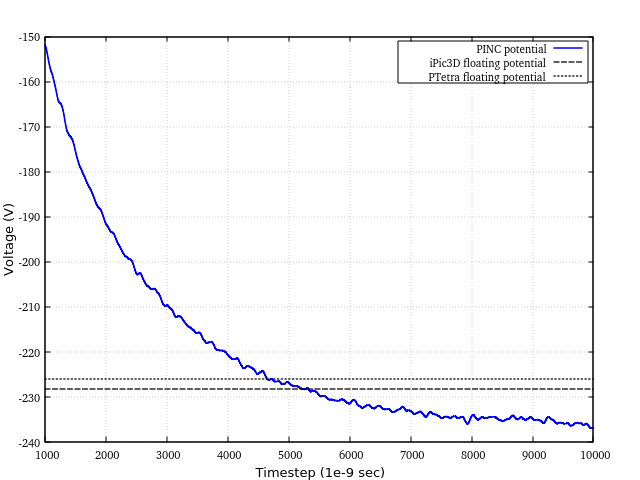
\includegraphics[scale=0.4]{figures/DECA/NoPhotoelectrons/pNoPH.png}
    \caption{Plot of the cubesat potential over time, in this case no photoelectrons are included and the cubesat is only charged by the ambient flowing plasma. The stippled horizontal lines show the floating potentials obtained by iPic3D and PTetra for the same simulation setup}
    \label{fig:pNoPH}
\end{figure}
\raggedbottom
Figure \ref{fig:pNoPH} shows a time series plot of the cubesat potential relative to the upstream plasma defined as ground. As the object charges over time, and the potential becomes more and more negative, more electrons are diverted away from the cubesat thereby slowing the rate of charging. The two horizontal lines in the figure show the computed floating potential found by iPic3D and PTetra; the floating potential found using PINC is more negative, and accurate to both results found by iPic3D and PTetra within a 4\% margin. Increasing the number of computational particles would reduce this inaccuracy, additionally due to the dimensions of the computational cells, the cubesat simulated in PINC has a smaller volume than the $1 m^3$ cubesat simulated by Deca et al. leading to further inaccuracies. 


\begin{figure}[H]
    \centering
    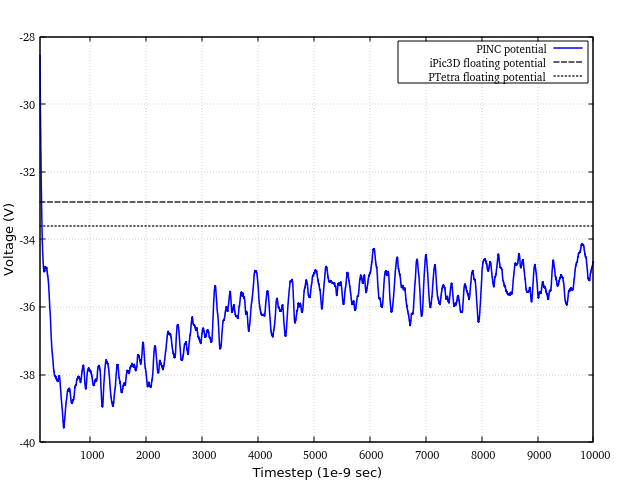
\includegraphics[scale=0.4]{figures/DECA/PhotoelectronsInjectionByCellFilling/pCellFill.png}
    \caption{Plot of the cubesat potential over time, in this case photoelectrons are injected into the domain using the adjacent cell filling method. The stippled horizontal lines show the floating potentials obtained by iPic3D and PTetra for the same simulation setup}
    \label{fig:pCellFill}
\end{figure}

Figure \ref{fig:pCellFill} shows the timeseries of the cubesat potential when photoemission using the cell filling algorithm is included. The potential stabilizes after approximately 5,000 timesteps before it begins to oscillate steadily with an amplitude of approximately 1 Volt around a steady state value. The first hundred timesteps are cut from the plot, to better show this oscillation. Comparisons of the cubesat potentials for the different injection algorithms are averaged over time after 5,000 timesteps to remove these fluctuations and give a better sense of the accuracy of each algorithm relative to the floating potentials found with iPic3D and PTetra.

\begin{figure}[H]
    \centering
    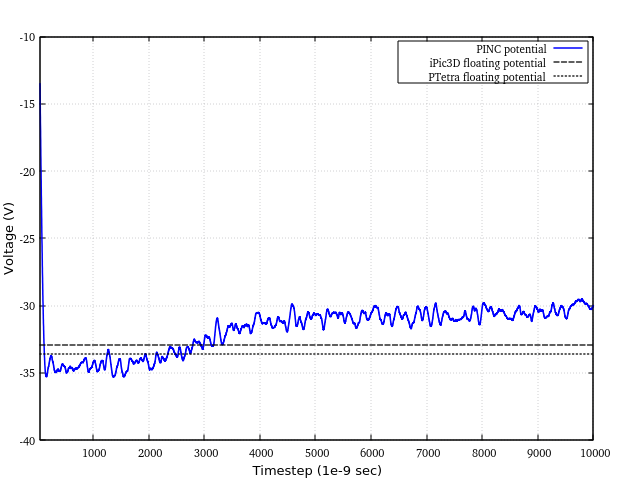
\includegraphics[scale=0.4]{figures/DECA/PhotoelectronInjectionByRotationMatrix/pRotMat.png}
    \caption{Plot of the cubesat potential over time, in this case photoelectrons are injected into the domain using equation \eqref{eq:injection} with velocity sampled from the univariate Maxwellian distribution and rotated using equation \eqref{eq:rotMatFull}. The stippled horizontal lines show the floating potentials obtained by iPic3D and PTetra for the same simulation setup}
    \captionsetup{belowskip=5pt}
    \label{fig:pRotMat}
\end{figure}

The timeseries plot of the cubesat potential in Figure \ref{fig:pRotMat} includes ambient plasma charging, and photoelectron charging where photoelectrons are emitted using the rotation matrix method. The oscillations around a steady state value are of the same amplitude as in figure \ref{fig:pCellFill}, but a less negative floating potential is predicted. Since the rotation matrix injection algorithm is based on a particle push of the sampled particle velocity distribution, this might be explained due to a higher concentration of photoelectrons near the cubesat surface as opposed to in the cell filling case. With a higher local density of electrons, the forces between the photoelectrons will be higher, thus imparting enough acceleration on a large enough mass of photoelectrons such that they pass the potential barrier formed by the photoelectron cloud. The higher number of "escaped" photoelectrons that are not reabsorbed by the cubesat then cause a less negative floating potential. 


\begin{figure}[H]
    \centering
    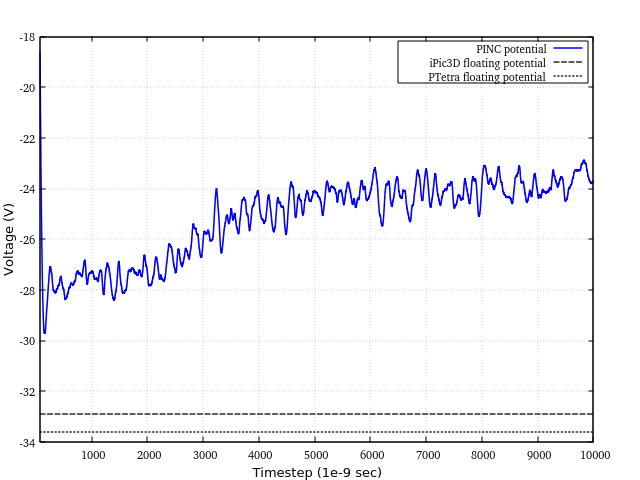
\includegraphics[scale=0.4]{figures/DECA/PhotoelectronInjectionByDoubleGauss/pDoubleGauss.png}
    \caption{Plot of the cubesat potential over time, in this case photoelectrons are injected into the domain using equation \eqref{eq:injection} and sampling the surface normal and tangential velocities separately. The stippled horizontal lines show the floating potentials obtained by iPic3D and PTetra for the same simulation setup}
    \label{fig:pDoubleGauss}
\end{figure}

\raggedbottom

Figure \ref{fig:pDoubleGauss} shows the timeseries plot of the cubesat potential where photoelectrons are injected into the computational domain by a particle push based on sampling a univariate and bivariate Maxwellian velocity distribution. This injection algorithm diverges by far by the largest amount from the floating potentials found using the iPic3D and PTetra codes. The large difference in floating potential, and the floating potential being the least negative, suggests photoelectrons injected with this algorithm have higher kinetic energy than photoelectrons injected using the two other algorithms. It could also be the case that higher densities of photoelectrons resulting from the particle push tangentially away from the surface, force more electrons away from the cubesat that are then not reabsorbed.

\newpage

\begin{table}[H]
%\centering
\begin{tabular}{p{4cm}|p{3cm}|p{3cm}|p{3cm}}
\toprule
\toprule
Photoelectron injection method & Floating potential & Percentage difference from iPic3D & Percentage difference from PTetra \\
\midrule
No photoelectrons & -233.242 & 2.21 \% & 3.20\% \\[1mm]
Cell filling & -35.31 & 7.33 \% & 5.09 \% \\[1mm]
Rotation matrix  & -30.61 & 6.96 \% & 8.90 \% \\[1mm]
Double gaussian sample & -24.03 & 26.96 \% & 28.48 \% \\[1mm]
\bottomrule
\bottomrule
\end{tabular}
\caption{Comparison of floating potentials found with iPic3D and PTetra, with the average potential of the cubesat from timestep 5,000 to timestep 10,000}
\label{tab:floatingPsummary}
\end{table}

\vspace{2cm}
Table \ref{tab:floatingPsummary} is a summary of the floating potentials computed using the injection algorithms I developed for this thesis. The "No photoelectrons" case give a baseline for differences in object charging when comparing PINC to iPic3D and PTetra. There is overall good agreement with the three codes in this simplest case, with only a 2.21 \% absolute difference in the floating potentials found between PINC and iPic3D.

These errors can be reduced by decreasing the tolerance of the solver used to compute the capacitance matrix in PINC, and reducing particle noise by increasing the number of computational particles introduced in the domain, at the cost of longer simulation times. 

Both the cell filling and rotation matrix injection algorithms are fairly close to values found by deca et al. when ambient plasma charging and photoemission are both included. The difference in computed floating potentials could again be reduced by setting a stricter tolerance for the multigrid solver in PINC, and increasing the number of computational particles used in the simulations. 


\subsection{Photoelectron cloud and wake formation}

\begin{figure}[H]
  \begin{subfigure}[b]{0.61\textwidth}
    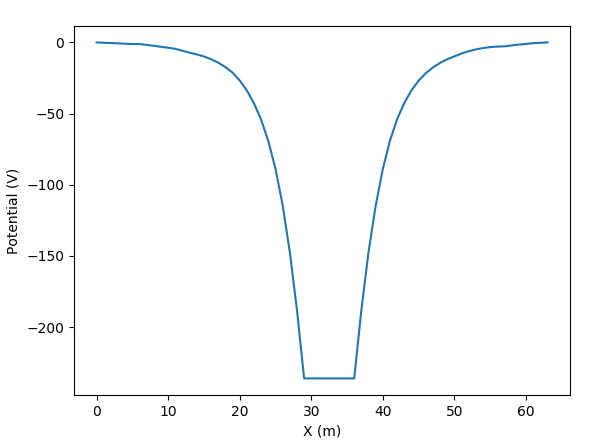
\includegraphics[width=\textwidth]{figures/DECA/NoPhotoelectrons/potentialAlongX.PNG}
    \caption{Potential along x axis}
    \label{fig:noPHalongX}
  \end{subfigure}
  \begin{subfigure}[b]{0.61\textwidth}
    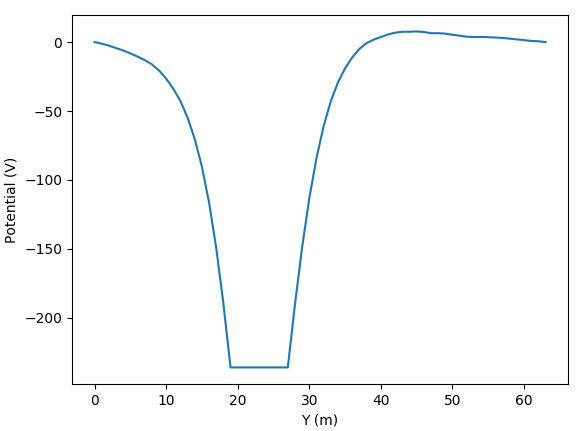
\includegraphics[width=\textwidth]{figures/DECA/NoPhotoelectrons/potentialAlongY.PNG}
    \caption{Potential along y axis}
    \label{fig:noPHalongY}
  \end{subfigure}
  \label{fig:NOPH}
  \caption{Potential profile along direction of flow (+Y axis), and along direction of light travelling from the sun (+X axis) when photoemission is omitted from the simulation, each line passes through the centre of the cubesat}
\end{figure}

In figures \ref{fig:noPHalongX}, and \ref{fig:noPHalongY} we have plotted the potential in Volts along the axis of drift, and along the axis of the sun through the centre of the cubesat at timestep 10,000. The spatial X-axis of each plot is multiples of the computational cell step size, in this case 0.15625 meters. 

The only charging mechanism included is the charging due to the ambient flowing plasma and is included as a baseline test to check the implementation of the capacitance matrix method in PINC and so that differences due to the photoemission implemented in this thesis may be singled out from the rest of the implementation of PINC.

No potential barrier can be seen in figure \ref{fig:noPHalongX}, and the plot is symmetric about the centre of the cubesat. In figure \ref{fig:noPHalongY} the potential relative to the upstream plasma rises above 0 behind the cubesat as expected due to the formation of an ion wake.


\begin{figure}[H]
  \begin{subfigure}[b]{0.6\textwidth}
    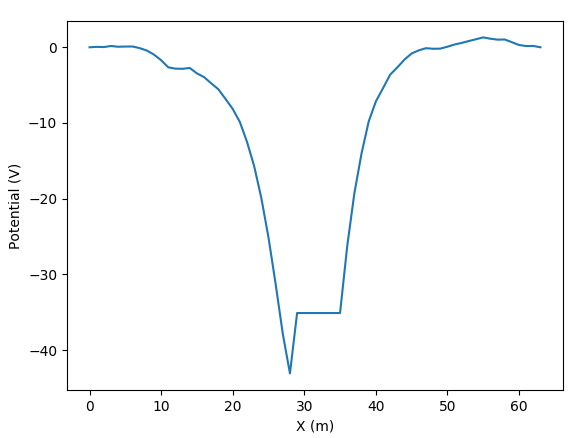
\includegraphics[width=\textwidth]{figures/DECA/PhotoelectronsInjectionByCellFilling/potentialAlongX.PNG}
    \caption{Potential along X axis}
    \label{fig:CellFillAlongX}
  \end{subfigure}
  %
  \begin{subfigure}[b]{0.6\textwidth}
    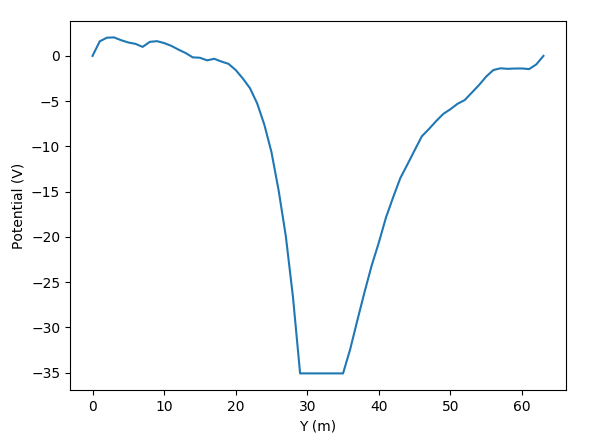
\includegraphics[width=\textwidth]{figures/DECA/PhotoelectronsInjectionByCellFilling/potentialAlongY.PNG}
    \caption{Potential along Y axis}
    \label{fig:CellFillAlongY}
  \end{subfigure}
  \label{fig:CELLFILL}
  \caption{Potential profile along direction of flow (+Y axis), and along direction of light travelling from the sun (+X axis) where photoelectrons are injected into the domain by randomly distributing the electrons uniformly into the cells adjacent to the emitting object surfaces, each line passes through the centre of the cubesat}
\end{figure}

Figure \ref{fig:CellFillAlongX} and \ref{fig:CellFillAlongY} include photoemission as a charging mechanism, where the cell filling algorithm in section \cref{subsec:injection} has been used to inject photoelectrons. Figure \ref{fig:CellFillAlongX} clearly shows a potential barrier forming in front of the object where the photoelectron cloud has formed. Figure \ref{fig:CellFillAlongY}, unlike figure \ref{fig:noPHalongY}, shows no ion wake forming behind the cubesat along the drift axis, likely due to photoelectrons reflecting off the potential barrier and drifting behind the cubesat.  

\begin{figure}[H]
  \begin{subfigure}[b]{0.6\textwidth}
    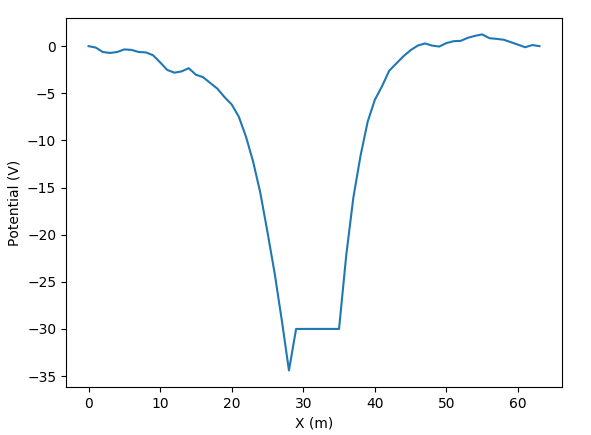
\includegraphics[width=\textwidth]{figures/DECA/PhotoelectronInjectionByRotationMatrix/potentialAlongX.PNG}
    \caption{Potential along X axis}
    \label{fig:RotMatAlongX}
  \end{subfigure}
  %
  \begin{subfigure}[b]{0.6\textwidth}
    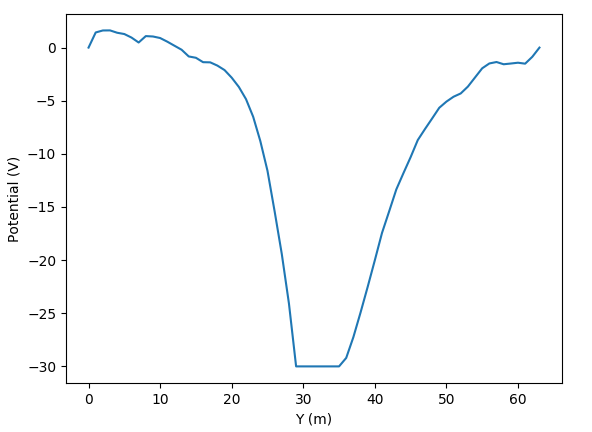
\includegraphics[width=\textwidth]{figures/DECA/PhotoelectronInjectionByRotationMatrix/potentialAlongY.PNG}
    \caption{Potential along Y axis}
    \label{fig:RotMatAlongY}
  \end{subfigure}
  \label{fig:RotMatAlong}
  \caption{Potential profile along direction of flow (+Y axis), and along direction of light travelling from the sun (+X axis) where photoelectrons are emitted using the rotation matrix algorithm and a partial particle push from object surface, each line passes through the centre of the cubesat}
\end{figure}

\raggedbottom


In figures \ref{fig:RotMatAlongX} and figure \ref{fig:RotMatAlongY} photoelectrons are injected by a partial particle push. The surface normal velocity is sampled from a univariate Maxwellian velocity distribution, then rotated by a random rotation tensor before the particle is pushed from the surface based on the computed velocity vector. The potential barrier in figure \ref{fig:RotMatAlongX} is smaller than found in figure \ref{fig:CellFillAlongX}, possibly due to more photoelectrons managing to escape the forming photoelectron cloud based on the random particle push, or due to the size of the computational cell: Refining the computational grid, and reducing the volume of the computational cells would likely decrease the difference in the potential barrier formed for the two cases. 


\begin{figure}[H]
  \begin{subfigure}[b]{0.6\textwidth}
    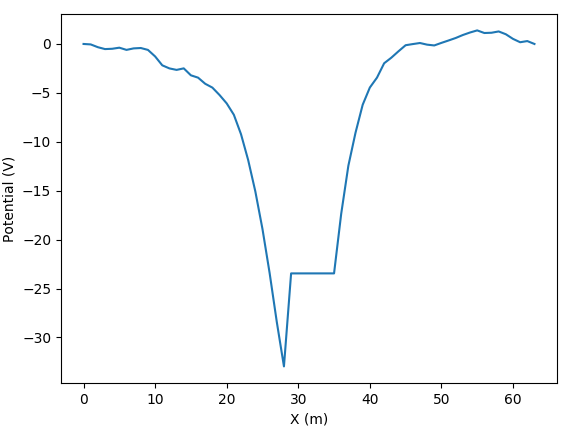
\includegraphics[width=\textwidth]{figures/DECA/PhotoelectronInjectionByDoubleGauss/potentialAlongX.PNG}
    \caption{Potential along X axis}
    \label{fig:DoubleGaussAlongX}
  \end{subfigure}
  %
  \begin{subfigure}[b]{0.6\textwidth}
    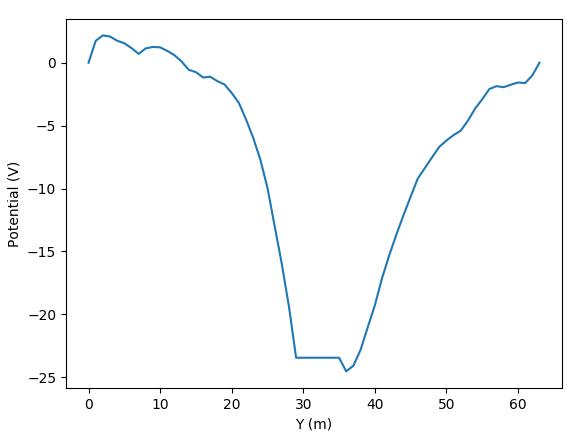
\includegraphics[width=\textwidth]{figures/DECA/PhotoelectronInjectionByDoubleGauss/potentialAlongY.PNG}
    \caption{Potential along Y axis}
    \label{fig:DoubleGaussAlongY}
  \end{subfigure}
  \label{fig:DoubleGaussAlong}
  \caption{Potential profile along direction of flow (+Y axis), and along direction of light travelling from the sun (+X axis) where photoelectrons are injected into the domain by a partial, random, particle push. Surface normal velocity and tangential surface velocity is sampled separately. Each line passes through the centre of the cubesat}
\end{figure}


Figures \ref{fig:DoubleGaussAlongX} and \ref{fig:DoubleGaussAlongY} plot potential profiles where photoelectrons are emitted similarly to the rotation matrix algorithm, but where the three dimensional particle velocity vectors are sampled in both the surface normal and tangential directions separately. Figure \ref{fig:DoubleGaussAlongX} shows the deepest potential well out of all the injection algorithms, but the least negative floating potential. 

A potential reason for this, is that the double sampling method increases the average kinetic energy of the emitted photoelectrons to a point where not all the photoelectrons return to the surface of the object and become reabsorbed. Figure \ref{fig:DoubleGaussAlongY} also shows another small barrier directly behind the cubesat along the direction of drift. 

This suggest that particles pushed based on the two samplings of velocity have higher tangential velocities in the photoelectrons than when injected using the other two algorithms, causing electrons to accumulate downstream of the object.

\todo{Sample pop file to check if electrons are Maxwellian? Can use the plot python script called VelDistributionSingle.py}

Based on the relative accuracy as shown in table \ref{tab:verificationPla} when compared to the two other PIC codes, an accurate reproduction of the expected physics, and the lower computational complexity as compared to the rotation matrix algorithm, I selected the cell filling algorithm as the injection algorithm to use when simulating MMO in its orbit around Mercury.


\section{Mercury Magnetospheric Orbiter simulation setup}
The MMO is one of the two spacecraft making up the joint European Space Agency (ESA) and Japan Aerospace Exploration Agency (JAXA) BepiColombo mission. The principal scientific goals of the MMO spacecraft is to investigate the plasma environment around Mercury as well as the interaction between the planets intrinsic magnetic field and the solar wind  \parencite{Benkhoff2009} \parencite{Saito2010}. 

Among the scientific instruments carried onboard the MMO, of special relevance to this thesis is the Mercury Plasma Particle Experiment (MPPE): The MPPE instrument package carries sensors for measuring plasma electrons and ions, as well as high energy particle sensors \parencite{Saito2010}. These sensors are highly sensitive to variations in the plasma density around the device, thus simulating how charging effects of the MMO spacecraft affects density measurements of these sensors is an important aspect of analyzing the data MMO will send back to Earth.

In this section, I outline aspects of the design of MMO relevant to an accurate simulation of charging phenomena, the plasma and numerical parameters used in the simulation, as well as outline the different numerical experiments that were run as part of this thesis to investigate the charging behaviour of the spacecraft while in orbit around Mercury.  


\subsection{MMO design}

The basic geometric shape of the MMO spacecraft is that of an octagon that can be surrounded by a 1.8 meter circle. The height of the octagon is 0.9 meters, with an upper section covered in both solar cells and second surface mirror (SSM), and the lower section only covered by SSM. The plasma particle instruments are situated inside this octagon, with their sensors placed on the surface panels of the octagon. Two 5 meter long booms extend from opposite sides of the spacecraft on which flux gate magnetometers are placed \parencite{Yamakawa2008}.

With these dimensions in mind, the MMO can be approximated by stacking voxels. A trade off must be made between the number of voxels used. A high number of voxels increases the accuracy of the object model, but requires longer compute times as the computational cell size decreases. For plasmas with relatively low densities, like the plasma found within Mercury's magnetosphere, coarser approximations with lower number of voxels is possible since the debye length is often significantly longer than the characteristic length of the spacecraft. 

\begin{figure}[H]
    \centering
    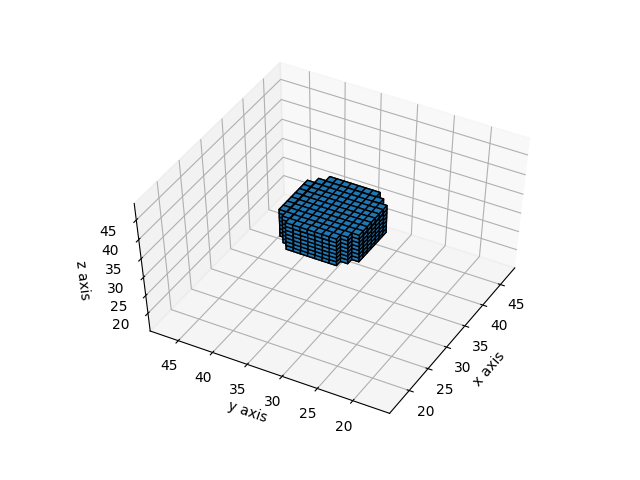
\includegraphics[scale=0.6]{figures/ReferenceFigures/MMO_no_booms_64.png}
    \caption{Voxelized approximation of MMO without booms in a 10 meter cubical computational domain with 64 grid points along each dimension. The plot ranges have been reduced to better display individual voxels}
    \label{fig:MMOnoBooms}
\end{figure}

\begin{figure}[H]
    \centering
    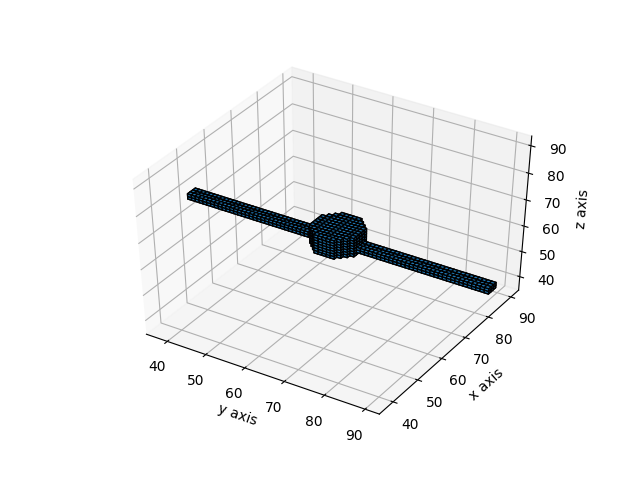
\includegraphics[scale=0.6]{figures/ReferenceFigures/MMO_with_booms.png}
    \caption{Voxelized approximation of MMO without booms in a 10 meter cubical computational domain with 128 grid points along each dimension. The plot ranges have been reduced to better display individual voxels}
    \label{fig:MMOWithBooms}
\end{figure}

\newpage


Figures \ref{fig:MMOnoBooms} and figure \ref{fig:MMOWithBooms} show two voxelized approximations of the MMO spacecraft, with and without the booms carrying the flux gate magnetometers. The high gain antenna and the wire antenna used to measure the electrical field have been discarded. These features are very thin, and would therefore increase the number of computational cells in the global domain to an untenable size. Both voxelizations were created by first constructing the objects in the CAD software suite Fusion 360, meshing the resulting object, and finding the voxels of the resulting mesh using a flood filling algorithm. The final voxelized version of both versions of the MMO used 8 cells over the diameter of the octagon shape of the MMO body. This allowed the shape of the spacecraft and the thickness of the booms to be resolved adequately, and allowed for a computational domain of several Debye lengths while keeping the total number of computational cells low enough for a full simulation to complete within a few days with parallelization.

\subsection{Magnetospheric and numerical parameters}

Two spacecraft have visited Mercury at the time of writing. The first spacecraft to do so was the Mariner 10 spacecraft, performing three fly-bys of the planet, equipped both with plasma detectors and magnetometers to study the properties of Mercury's magnetic field and its interaction with the solar wind plasma \insertref{MESSENGER and Mariner 10 flyby observations of magnetotail structure and dynamics at Mercury}. A longer observation mission, the MESSENGER spacecraft, entered into orbit around Mercury as the first spacecraft to do so. It orbited the planet from 2011 to 2015 in a highly eccentric orbit, collecting data all the while on the plasma conditions of the planets magnetosphere, magnetotail and the intrinsic magnetic field of the planet.

In this thesis, I have used a combination of data gathered from the MESSENGER mission, as well as MHD simulations of solar wind interaction with the magnetosphere of Mercury, to simulate the charging of the MMO spacecraft. Several assumptions were made in carrying out this analysis; first of all, the MMO spacecraft is spin-stabilized \parencite{Yamakawa2008} to reduce thermal load with its spin axis aligned along the magnetic dipole axis of Mercury. Because of the small timescales of charging relative to the rotational rate of the spacecraft, I have assumed an irrotational body fixed reference frame for the PINC simulations. Furthermore, MMO will orbit Mercury in a polar orbit with a period of 9.3 hours \insertref{ESA fact sheet}. As such, I chose to simulate the charging of the spacecraft close to the periapsis of MMO's orbit. Specifically, when the spacecraft is over Mercury's magnetic south pole where the plasma density is relatively high and exposed to direct sunlight. The distance of Mercury to the sun was also assumed to be the same as used in \parencite{Benna2009} such that the photon flux experienced by the MMO can be computed accurately. 


\begin{table}[H]
    \centering
    \begin{tabular}{c|c}
        \toprule
        \toprule
        Parameter & Value \\
        \midrule
        $Timesteps$ & 10,000 \\
        dt & $5 \times 10^{-9} (10^{-8})$ \\
        dx, dy, dz & 0.225 m \\
        $n_x, n_y, n_z$ & 128 \\
        $n_0$ & $1 \times 10^8 m^{-3}$ \\
        $m_e$ & $9.10938356 \times 10^{-31}$ kg\\
        $m_i$ & $1.67262192 \times 10^{-27}$ kg\\
        $\vb{B}_0$ & [-8.8, 0, -99.6] nT\\
        $v_{drift}$ & $1 \times 10^5$ m/s\\
        $v_{th,e}$ & 4193011.62 m/s\\
        $v_{th,i}$ & 87538.91 m/s\\
        $n_{p,com}$ & 50 pc\\
        $r_{sc}$ & $5.6847 \times 10^{10} m$\\
        $\overline{Y}_{ph}$ & $ 1 \times 10^{-3}$ \\
        $A_{ph}$ & 1.62 (3.87) \\
        $W$ & 4.2 eV \\
        \bottomrule
        \bottomrule
    \end{tabular}
    \caption{Magnetospheric plasma parameters, MMO specific parameters, and numerical parameters used in MMO simulations}
    \label{tab:PlasmaParamMMO}
\end{table}

Table \ref{tab:PlasmaParamMMO} summarizes all relevant parameters used in the charging simulation of the MMO spacecraft. The plasma density and thermal velocity values were extracted from the MHD simulation plots given in the paper by Benna et al. modelling the magnetosphere of Mercury at the first MESSENGER flyby. The intrinsic magnetic field of Mercury is dominantly dipolar, with a dipole tilt to the rotational axis constrained to being less than $\ang{5}$ \parencite{Anderson2010}. Mercury's rotational axis is tilted 2 minutes of arc with respect to its orbital plane \parencite{Rothery2015}, and has a external field strength of about $100 nT$ at the north cusp \parencite{Anderson2010}. Using the maximum dipole axis tilt angle, the value for the magnetic field $\vb{B}_0$ in table \ref{tab:PlasmaParamMMO} is then given in the Mercury solar orbital (MSO) coordinates. 

The distance from the MMO to the sun $r_{sc}$ was computed using the Jet Propulsion Lab (JPL) ephemeris system HORIZONS and setting the time of the ephemeris to the day of the first MESSENGER Mercury fly-by.

The parameter $\overline{Y}$ is the photoelectron yield per incoming photon and averaged over the range of photon energies that cause photoemission for MMO. Here we have assumed the MMO to be covered by Multi Layer Insulation (MLI), a thermal insulation covering consisting of several layers of plastic coated with an outer layer of Aluminium. The average photoelectron yield of Aluminium and its work function were found in \parencite{Feuerbacher1972}, the yield parameter used is dependent on the reflectance of the Aluminium, and as such the reflectance is not included as a separate parameter. 

The SSM panels that cover the MMO are composed of silver films which have a slightly higher, but similar, work function to that of Aluminium. The parameter $A_{MM0}$ denotes the sunlit area of the MMO with and without the magnetometer booms. Since the booms account for a significant part of the sunlit surface area of the spacecraft the properties of Aluminium was used for simulations both with and without the booms.

\newpage
%\section{Data analysis tools}